
% !TEX root = DesignDocument.tex

\chapter{Design  and Implementation}
This section is used to describe the design details for each of the major components 
in the system.    Note that this chapter is critical for all tracks.  Research tracks would do experimental design here where other tracks would include the engineering design aspects.    This section is not brief and requires the necessary detail that 
can be used by the reader to truly understand the architecture and implementation 
details without having to dig into the code.    Sample algorithm:  Algorithm~\ref{alg1}.  This algorithm environment is automatically placed - meaning it floats.   You don't have to worry about placement or numbering.  

\begin{algorithm} [tbh]                     % enter the algorithm environment
\caption{Calculate $y = x^n$}          % give the algorithm a caption
\label{alg1}                           % and a label for \ref{} commands later in the document
\begin{algorithmic}                    % enter the algorithmic environment
    \REQUIRE $n \geq 0 \vee x \neq 0$
    \ENSURE $y = x^n$
    \STATE $y \Leftarrow 1$
    \IF{$n < 0$}
        \STATE $X \Leftarrow 1 / x$
        \STATE $N \Leftarrow -n$
    \ELSE
        \STATE $X \Leftarrow x$
        \STATE $N \Leftarrow n$
    \ENDIF
    \WHILE{$N \neq 0$}
        \IF{$N$ is even}
            \STATE $X \Leftarrow X \times X$
            \STATE $N \Leftarrow N / 2$
        \ELSE[$N$ is odd]
            \STATE $y \Leftarrow y \times X$
            \STATE $N \Leftarrow N - 1$
        \ENDIF
    \ENDWHILE
\end{algorithmic}
\end{algorithm}
Citations look like~\cite{Choset:2005:PRM, arkin2009governing, lavalle2006}  and~\cite{wiki:asimo,lumelsky:1987, nolfi2000evolutionary}.  These are done automatically.  Just fill in the database {\tt designrefs.bib} using the same field structure as the other entries.  Then pdflatex the document, bibtex the document and pdflatex twice again.  The first pdflatex creates requests for bibliography entries.
The bibtex extracts and formats the requested entries.  The next pdflatex puts them in order and assigns labels.  The final pdflatex replaces references in the text with the assigned labels.
The bibliography is automatically constructed.  
 
 \section{Architecture and System Design}
 This is section will detail the overall system design and general architecture of Crowd Control. The software was designed in such a way that minimizes dependency from third-party services such as Sinch and Parse.
 
 \subsection{Design Selection}
Sprint 1 was centered around designing of the database schema and the general system architecture. Bowtaps produced various high-level designs on both the front-end and back-end of the system that were deeply inspected before deciding on our current implementation.

\subsubsection{Early Design Ideas}
The original database design for Crowd Control consisted of three tables with associated data. Though this design provided a good sense of direction and foundation to build upon, it eventually would need to expand as Crowd Control's feature set expanded. See Figure~\ref{EarlyDBSchema} below.

	\begin{figure}[tbh]
	\begin{center}
	\fbox{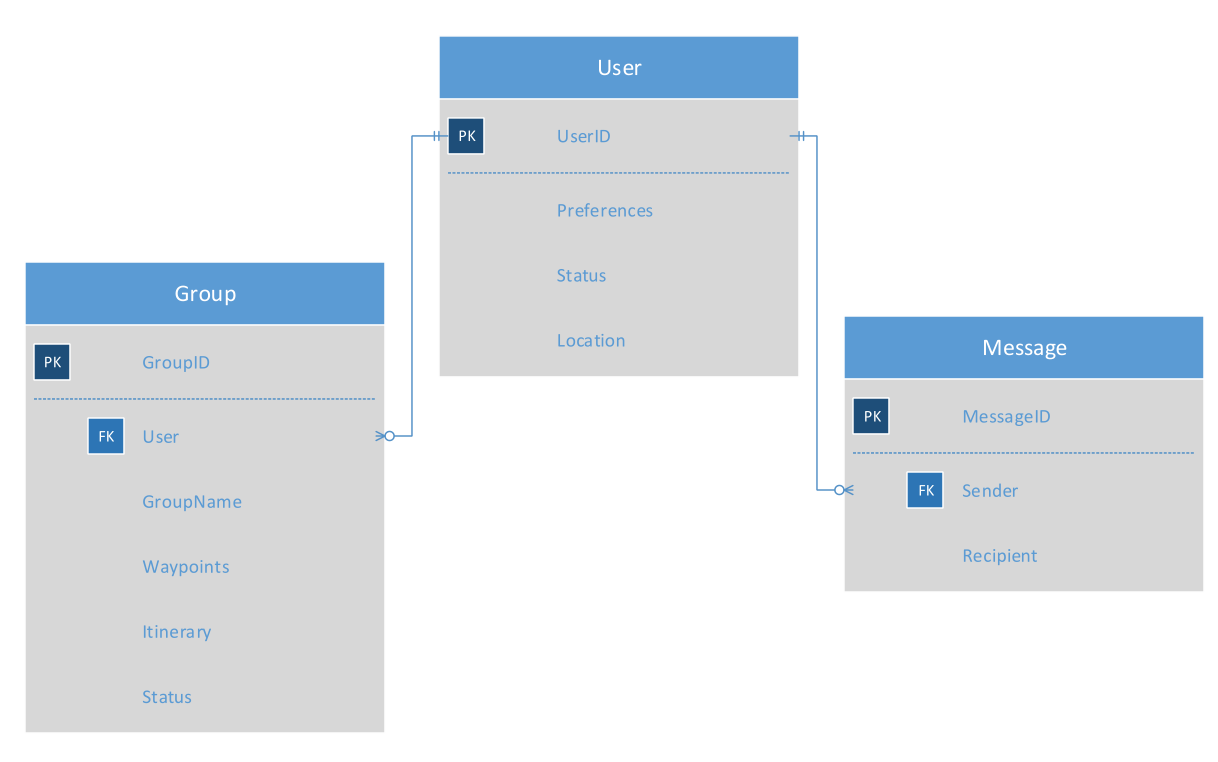
\includegraphics[scale=.5]{Additional/DesignPictures/CC_dbSchema1.PNG}}
	\end{center}
	\caption{Early database schema. \label{EarlyDBSchema}}
	\end{figure}

Another caveat to this design is the failure to differentiate between public and private user data. In Crowd Control, each user has data that is private to that user, such as their email and password. However, there is also a set of public data that can be viewed by other users, such as their display name or their location. This iteration of the schema only has one user entity, that stores their information. A small lack of understanding about Parse's no-SQL implementation lead us to improperly design our entities in this way. It was later deemed that this separation between front-facing and hidden user data entities was necessary in terms of ease-of-access and information privacy.

\subsubsection{Improvements to Early Designs}
In reflection of the shortcomings of the first design iteration, the database schema was restructured to better fit Crowd Control's needs. The current design consists of eight data tables,  shown in Figure~\ref{MidDBSchema} below. More entities were added to the overall schema. One such addition was a ``CCUser'' table to hold the public data associated with a user. It is important to note that the ``User'' table was left to hold a user's private data. Those changes and some additions resulted in the below schema. 

	\begin{figure}[tbh!]
	\begin{center}
	\fbox{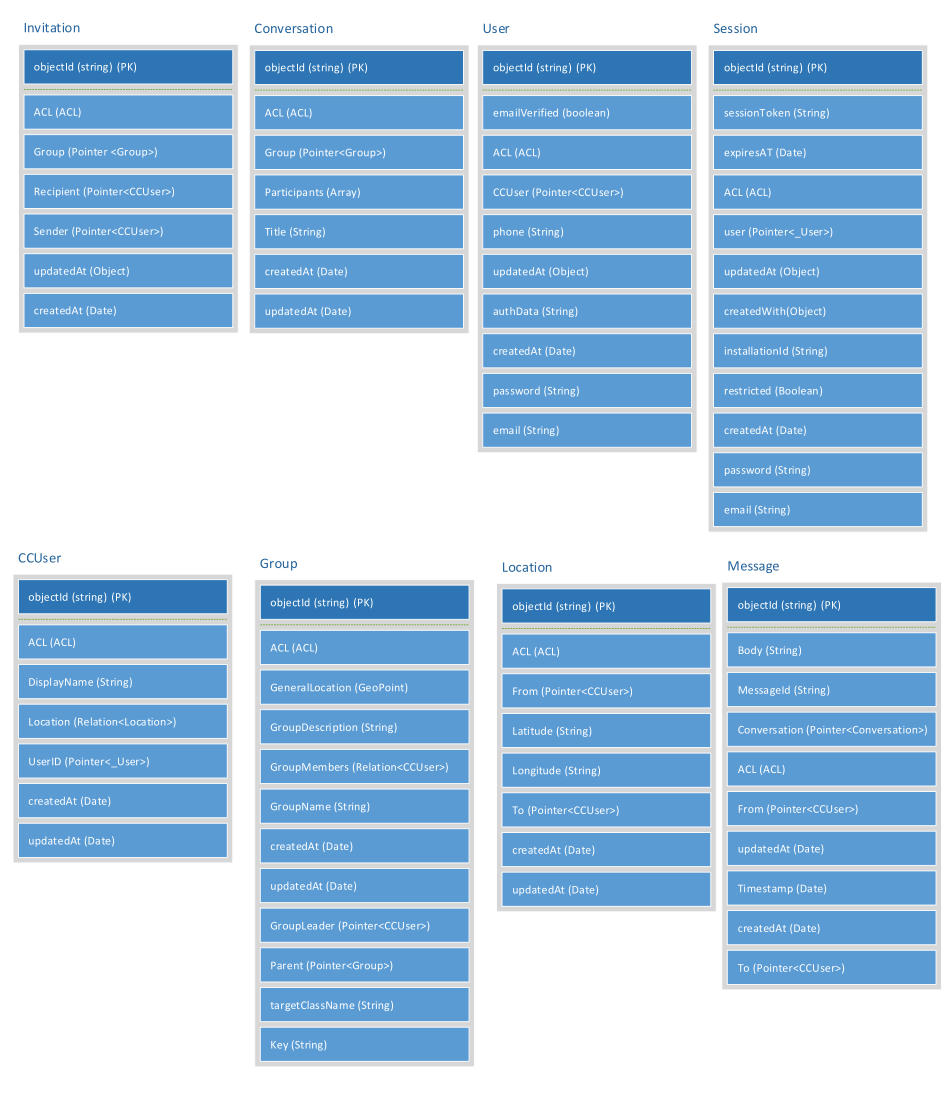
\includegraphics[scale=.65]{Additional/DesignPictures/CC_dbSchema2.PNG}}
	\end{center}
	\caption{Improved database schema. \label{MidDBSchema}}
	\end{figure}

 \subsection{Data Structures and Algorithms}
 TODO: Model classes and hierarchy? Perhaps irrelevant (see ``Classes below'')
 
 \subsection{Data Flow}
 TODO: Create Data Flow diagram of overall process
 
 
 \subsection{Communications}
 One of the core features to the Crowd Control app is communication amongst its users. To achieve this, some third-party services are used, which in turn communicate data between users. If a user wishes to send another user a message, that message is sent to the Parse back-end, and delivered to the recipient via the Sinch service. The basic communication overview is outlined below in Figure ~\ref{CommFlow}.
 
  	\begin{figure}[tbh]
	\begin{center}
	\fbox{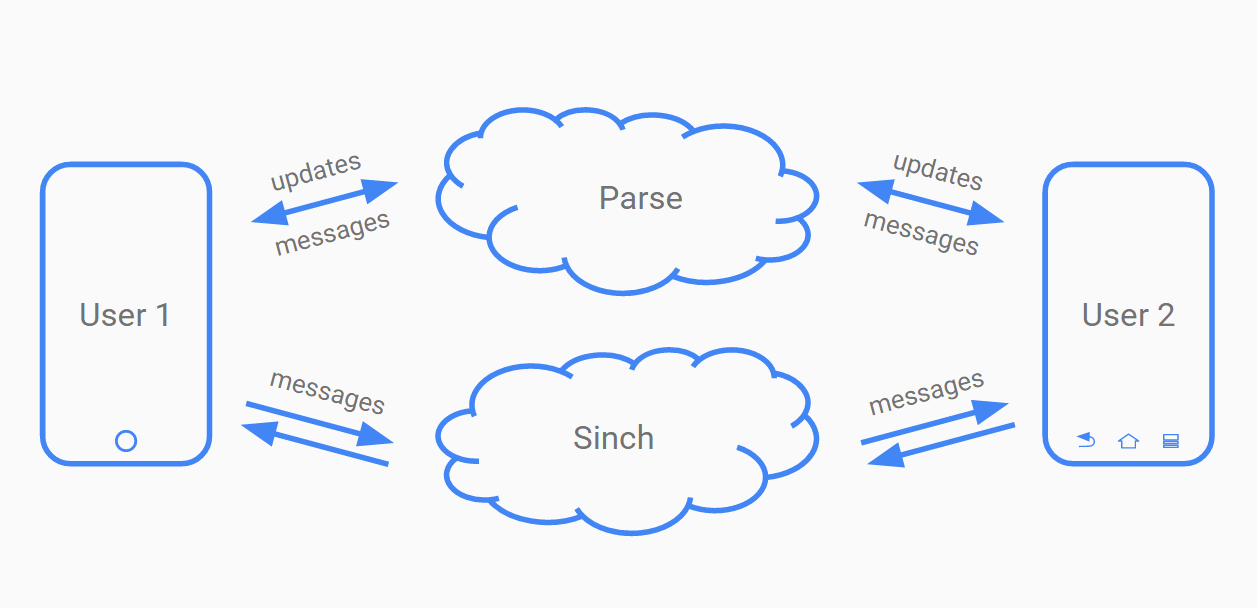
\includegraphics[scale=.5]{Additional/DesignPictures/CommFlow.PNG}}
	\end{center}
	\caption{Communication flow diagram. \label{CommFlow}}
	\end{figure}
 
 In addition to message-passing, various other data is being transfered from the users' devices. One such example is GPS data. Upon retrieval of a user's location, that value is stored in Parse, and able to be fetched by any group member that wishes to see that location. 

 \subsection{Classes}
 TODO: Include class hierarchy (models, base models, interfaces)
 \subsection{UML}
 TODO: UML diagram...can Android studio generate these via a plugin?
 
 \subsection{GUI}
 TODO: Overview of GUI design. Show differences in platform native ``look and feel''
 
 \subsection{MVVM, etc}
 TODO: Describe MVVM, create diagram laying our components in MVVM format

\section{Group Messaging }

\subsection{Technologies  Used}
\begin{itemize}
  \item Parse
  \item Sinch
\end{itemize}

\subsection{Component  Overview}
\begin{itemize}
  \item Send/receive messages to/from group members (many-to-many)
  \item Store messages in Parse (data persistence)
  \item Message transfer service is independent of carrier/device/platform
\end{itemize} 

\subsection{Phase Overview}
This is an extension of the Phase Overview above, but specific to this component. 
 It is meant to be basically a brief list with space for marking the phase status. 

\subsection{Architecture Diagram}
It is important to build and maintain an architecture diagram.  However, it may 
be that a component is best described visually with a data flow diagram. 

\subsection{Data Flow Diagram}
It is important to build and maintain a data flow diagram.  However, it may be 
that a component is best described visually with an architecture diagram. 

\subsection{Design Details} - NOTE: Code block probably irrelevant here. Will remove later.
This is where the details are presented and may contain subsections.   Here is an example code listing:
\begin{lstlisting}
#include <stdio.h>
#define N 10
/* Block
 * comment */
 
int main()
{
    int i;
 
    // Line comment.
    puts("Hello world!");
 
    for (i = 0; i < N; i++)
    {
        puts("LaTeX is also great for programmers!");
    }
 
    return 0;
}
\end{lstlisting}
This code listing is not floating or automatically numbered.  If you want auto-numbering, but it in the algorithm environment (not algorithmic however) shown above.

\section{Location Tracking }

\subsection{Technologies  Used}
\begin{itemize}
  \item Google Play Services / Apple Map Features
  \item Parse
\end{itemize}

\subsection{Component  Overview}
\begin{itemize}
  \item Track all group members in a map fragment
  \item Homing functionality on the user's location pin
  \item Sync group locations automatically (interval-based) and manually (on button-press)
\end{itemize}

\subsection{Phase Overview}
This is an extension of the Phase Overview above, but specific to this component. 
 It is meant to be basically a brief list with space for marking the phase status. 

\subsection{ Architecture  Diagram}
It is important to build and maintain an architecture diagram.  However, it may 
be that a component is best described visually with a data flow diagram. 

\subsection{Data Flow Diagram}
It is important to build and maintain a data flow diagram.  However, it may be 
that a component is best described visually with an architecture diagram. 


\subsection{Design Details}
This is where the details are presented and may contain subsections. 

\section{Group Management }

\subsection{Technologies  Used}
\begin{itemize}
  \item Parse
\end{itemize}

\subsection{Component  Overview}
\begin{itemize}
  \item Store group members in a group
  \item Incorporate a party leader to manage the group (has special priveledges)
  \item Create a group with specific attributes that can be changed by the leader
\end{itemize}

\subsection{Phase Overview}
This is an extension of the Phase Overview above, but specific to this component. 
 It is meant to be basically a brief list with space for marking the phase status. 

\subsection{ Architecture  Diagram}
It is important to build and maintain an architecture diagram.  However, it may 
be that a component is best described visually with a data flow diagram. 


\subsection{Data Flow Diagram}
It is important to build and maintain a data flow diagram.  However, it may be 
that a component is best described visually with an architecture diagram. 


\subsection{Design Details}
This is where the details are presented and may contain subsections. 


